\documentclass[notes]{subfiles}

\begin{document}
	\addcontentsline{toc}{section}{3.9 - Antiderivatives}
	\refstepcounter{section}
	\setcounter{section}{9}
	\fancyhead[RO,LE]{\bfseries \large\nameref{cs39}} 
	\fancyhead[LO,RE]{\bfseries \currentname}
	\fancyfoot[C]{{}}
	\fancyfoot[RO,LE]{\large \thepage}	%Footer on Right \thepage is pagenumber
	\fancyfoot[LO,RE]{\large Chapter 3.9}
	
\section*{Antiderivatives}\label{cs39}
	\subsection*{Before Class}
	\addcontentsline{toc}{subsection}{Before Class}
	\subsubsection*{Derivatives}
	\addcontentsline{toc}{subsubsection}{Derivatives}
		Before we begin with antiderivatives, let's collect a table of derivatives that we know.
		\begin{ex}
			Complete the table of derivatives:
			\showto{ins}{
				\begin{center}
				\tabulinesep = 4mm
				\begin{tabu} {| X[.75,c] | X[c] || X[.75,c] | X[c] |}\hline
					\textbf{Function}	& \textbf{Derivative}	& \textbf{Function}	& \textbf{Derivative} \\ \hline
					$c$				& $0$					& $x^n$				& $nx^{n-1}$ \\ \hline
					$\sin x$			& $\cos x$				& $\cos x$			& $-\sin x$ \\ \hline
					$\tan x$			& $\sec^2x$				& $\cot x$			& $-\csc^2x$ \\ \hline
					$\sec x$			& $\sec x\tan x$			& $\csc x$			& $-\csc x\cot x$\\ \hline
					$c\cdot f(x)$		& $c\cdot f'(x)$			& $f(x)\pm g(x)$		& $f'(x)\pm g'(x)$\\ \hline
					$f(x)\cdot g(x)$	& $f'(x)g(x) + f(x)g'(x)$	& $\dfrac{f(x)}{g(x)}$& $\dfrac{f'(x)g(x)-f(x)g'(x)}{[g(x)]^2}$\\ \hline
					$f(g(x))$		& $f'(g(x))\cdot g'(x)$		& 					& \\ \hline
				\end{tabu}
			\end{center}
			}
			
			\showto{st}{
				\begin{center}
					\tabulinesep = 2mm
					\begin{tabu}to .8\textwidth {| X[c] | X[c] || X[c] | X[c] |}\hline
						\textbf{Function}	& \textbf{Derivative}	& \textbf{Function}	& \textbf{Derivative} \\ \hline
										&					&					& \\
						$c$				&					& $x^n$				& \\
										&					&					& \\ \hline
										&					&					& \\
						$\sin x$			&					& $\cos x$			& \\
										&					&					& \\ \hline
										&					&					& \\
						$\tan x$			&					& $\cot x$			& \\
										&					&					& \\ \hline
										&					&					& \\
						$\sec x$			&					& $\csc x$			& \\
										&					&					& \\ \hline
										&					&					& \\
						$c\cdot f(x)$		&					& $f(x)\pm g(x)$		& \\
										&					&					& \\ \hline
										&					&					& \\
						$f(x)\cdot g(x)$	&					& $\dfrac{f(x)}{g(x)}$& \\
										&					&					& \\ \hline
										&					&					& \\
						$f(g(x))$		&					& 					& \\ 
										&					&					& \\ \hline
					\end{tabu}
				\end{center}
			}
		\end{ex}
		\newpage
		
	\subsubsection*{The Antiderivative}
	\addcontentsline{toc}{subsubsection}{The Antiderivative}
		\begin{defn}[Antiderivative]
			A function $F$ is called an \textbf{antiderivative} of $f$ on an interval $I$ if 
			\showto{ins}{
				\fbox{$F'(x) = f(x)$ for all $x\in I$}.  
			}
			\showto{st}{
				\blank{2}\\ \\\blank{2}.
			}
		\end{defn}
			
		\begin{ex}
			Find five antiderivatives for the function $f(x) = 2x$.
		\end{ex}
			\vs{1}
			
		\begin{question}
			How might we write the general antiderivative $F(x)$ for $f(x) = 2x$?  
		\end{question}
			\vs{1}
			
		\begin{ex}
			Find the most general antiderivative for the functions $f(x) = \cos x$, $g(x) = x^n$ ($n\geq 0$), and $h(x) = x^{-2}$.
		\end{ex}
			\vs{2}
			\newpage
			
		A table of useful antiderivatives is given below:
			\showto{ins}{
				\begin{center}
				\tabulinesep = 4mm
				\begin{tabu} {| X[.75,c] | X[c] || X[.75,c] | X[c] |}\hline
					\textbf{Function}	& \textbf{Antiderivative}	& \textbf{Function}	& \textbf{Antiderivative} \\ \hline
					$0$				& $0$					& $k$				& $kx$ \\ \hline
					$x^n$			& $\dfrac{x^{n+1}}{n+1}$		& $\sin x$			& $-\cos x$ \\ \hline
					$\cos x$			& $\sin x$				& $\sec^2 x$			& $\tan x$ \\ \hline
					$\csc^2 x$		& $-\cot x$			& $\sec x\tan x$		& $\sec x$\\ \hline
					$\cot x\csc x$		& $-\csc x$			& $c\cdot f(x)$		& $c\cdot F(x)$\\ \hline
					$f(x)\pm g(x)$		& $F(x)\pm G(x)$		& & \\ \hline
				\end{tabu}
			\end{center}
			}
			
			\showto{st}{
				\begin{center}
					\tabulinesep = 2mm
					\begin{tabu}to .8\textwidth {| X[c] | X[c] || X[c] | X[c] |}\hline
						\textbf{Function}	& \textbf{Antiderivative}	& \textbf{Function}	& \textbf{Antiderivative} \\ \hline
										&					&					& \\
						$0$				&					& $k$				& \\
										&					&					& \\ \hline
										&					&					& \\
						$x^n$			&					& $\sin x$			& \\
										&					&					& \\ \hline
										&					&					& \\
						$\cos x$			&				& $\sec^2 x$			& \\
										&					&					& \\ \hline
										&					&					& \\
						$\csc^2 x$			&				& $\sec x\tan x$			& \\
										&					&					& \\ \hline
										&					&					& \\
						$\cot x\csc x$		&					& $c\cdot f(x)$		& \\
										&					&					& \\ \hline
										&					&					& \\
						$f(x)\pm g(x)$		&					& 					& \\
										&					&					& \\ \hline
					\end{tabu}
				\end{center}
			}
		\begin{ex}
			$g'(x) = 3\sin x - \dfrac{9x^4-\sqrt[3]{x}}{x^2}$.  Find $g(x)$, the most general antiderivative of $g$.
		\end{ex}
			\vs{1}
			
		\begin{ex}
			Find $f$ if $f'(x) = x\sqrt{x}$ and $f(1) = 5$.
		\end{ex}
			\vs{1}
			\newpage
	\subsubsection*{Pre-Class Activities}
	\addcontentsline{toc}{subsubsection}{Pre-Class Activities}
		\begin{ex}
			Find the most general antiderivative of the following functions; check your answer by differentiation.
			\begin{enumerate}[(a)]
				\item $f(x) = 5x + 3$
					\vs{1}
					
				\item $f(x) = x(12x + 8)$
					\vs{1}
					
				\item $g(x) = \sqrt{5}$
					\vs{1}
					
				\item $h(x) = -3\sqrt{x} - 8\sqrt[3]{x}$
					\vs{1}
					
				\item $k(x) = \dfrac{6}{x^7}$
					\vs{1}
					
				\item $f(t) = \dfrac{5-4t^3 + 2t^6}{t^6}$
					\vs{1}
			\end{enumerate}
		\end{ex}
			\newpage
	
	\subsection*{In Class}
	\addcontentsline{toc}{subsection}{In Class}
		\begin{rmk}[General Antiderivative vs. Specific Antiderivative]
			A \emph{general antiderivative} takes the form \showto{ins}{$F(x) + C$} \showto{st}{\blank{2}}, while a \emph{specific} \showto{st}{\\ \\} \emph{antiderivative} takes the form \showto{ins}{$F(x)$} \showto{st}{\blank{1.5}}.  For a specific antiderivative, we must \showto{st}{\\ \\}have information about \showto{ins}{the value(s) of the original function.} \showto{st}{\blank{3.5}.}
		\end{rmk}
		\begin{ex}
			Find $f$ if $f''(x) = 12x^2+6x-4$, $f(0) = 4$, and $f(1) = 2$.
		\end{ex}
			\vs{1}
			
		\begin{ex}
			A particle moves in a straight line, and its acceleration is given by $a(t) = 3t+2$.  Its initial velocity is $v(0) = -3$ cm/s, and its initial displacement is $s(0) = 5$ cm.  Find the position function $s(t)$.
		\end{ex}
			\vs{1}
			\newpage
			
		\begin{ex}
			A ball is thrown upward with speed 24 ft/s from the edge of a cliff which is 432 ft above the ground.  Find its height above the ground $t$ seconds later.  When does it reach its maximum height?  When does it hit the ground?
		\end{ex}
			\vs{2.5}
			
		\begin{ex}
			Find the most general antiderivative of $f(x) = (x-5)^2$.
		\end{ex}
			\vs{1}
			
		\begin{ex}
			Find the most general antiderivative of $f(x) = \pi^2$.
		\end{ex}
			\vs{.5}
	
		\begin{ex}
			Find the most general antiderivative of $f(t) = 3\cos t - 4\sin t$.
		\end{ex}
			\vs{.5}
			\newpage
			
		\begin{ex}
			Find the most general antiderivative of $f(x) = 8\sqrt{x}-\sec x\tan x$.
		\end{ex}
			\vs{1}
			
		\begin{ex}
			Find $f$, if $f''(x) = \sin x + \cos x$, $f(0) = 3$, and $f'(0)= 4$.
		\end{ex}
			\vs{1}
		
		\begin{ex}
			The graph of $f$ passes through the point $(2,5)$, and the slope of its tangent line at $(x,f(x))$ is $3-4x$.  Find $f(1)$.
		\end{ex}
			\vs{2}
			\newpage
			
	\subsection*{After Class}		
	\addcontentsline{toc}{subsection}{After Class}
		\begin{ex}
			Find $g$, if $g'''(t) = 12+\cos t$.
		\end{ex}
			\vs{1}
		
		\begin{ex}
			A car is traveling at 60 mi/h when the brakes are fully applied, producing a constant deceleration of 20 ft/s$^2$.  What is the distance traveled before the car comes to a stop?
		\end{ex}	
			\vs{1}
			
		\begin{ex}
			The graph of a function is show below.  Make a rough sketch of an antiderivative $F$, if $F(0) = 1$.\\
			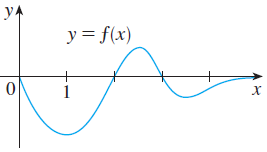
\includegraphics{3.9fig1}
		\end{ex}
			\vs{1.5}
	\clearpage
\end{document}